\chapter{Matrix theorem}


\section*{Adjacency matrix}

Let us describe a way to encode a given multigraph $G$ with $p$ vertexes by an $p{\times}p$ matrix.
First, enumerate the vertexes of the multigraph by numbers from $1$ to $p$;
such a multigraph will be called \index{labeled graph}\emph{labeled}. 
Consider the matrix $A=A_G$ with the component $a_{i,j}$ equal to the number of edges from the $i$-th vertex to the $j$-th vertex of $G$.

This matrix $A$ is called the \index{adjacency matrix}\emph{adjacency matrix} of $G$.
Note that $A$ is \index{symmetric matrix}\emph{symmetric}; that is, $a_{i,j}=a_{j,i}$ for any pair $i,j$.
Also, the diagonal components of $A$ vanish; that is, $a_{i,i}=0$ for any $i$.

{

\begin{wrapfigure}{o}{28 mm}
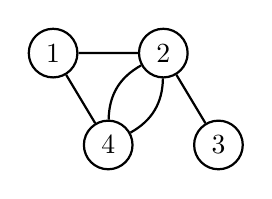
\begin{tikzpicture}[scale=1.4,
  thick,main node/.style={circle,draw,font=\sffamily\bfseries,minimum size=3mm}]

  \node[main node] (1) at (0,15/6) {$1$};
  \node[main node] (2) at (1,15/6){$2$};
  \node[main node] (11) at (1.5,10/6){$3$};
  \node[main node] (12) at (.5,10/6) {$4$};

  \path[every node/.style={font=\sffamily\small}]
  
   (1) edge node{}(2)
   (1) edge node{}(12)
   (2) edge[bend left] node{}(12)
   (2) edge[bend right] node{}(12)
   (2) edge node{}(11)
   (12) edge node{}(12);
\end{tikzpicture}
\end{wrapfigure}


For example, for the labeled multigraph $G$ shown on the diagram, we get the following adjacency matrix:
\[A=\left(
\begin{matrix}
0&1&0&1
\\
1&0&1&2
\\
0&1&0&0
\\
1&2&0&0
\end{matrix}
\right).\]

}

\begin{thm}{Exercise}
Let $A$ be the adjacency matrix of a labeled multigraph.
Show that the components $b_{i,j}$ of the $n$-th power $A^n$ is the number of walks of length $n$ in the graph from vertex $i$ to vertex $j$. 
\end{thm}

\parit{Hint:} Use induction on $n$.

\section*{Kirchhoff minor}

In this section we construct a special matrix, called {}\emph{Kirchhoff minor}, associated with a pseudograph,
and we discuss its basic properties.
This matrix will be used in the next section in a formula for the number of spanning trees in a pseudograph~$G$.
Since the loops do not change the number of spanning trees, we can remove all of them.
In other words, we can (and will) always assume that $G$ is a multigraph. 

Fix a multigraph $G$ and consider its adjacency matrix $A=A_G$;
it is a $p{\times}p$ symmetric matrix with zeros on the diagonal.

\begin{enumerate}
\item Revert the signs of the components of $A$ and exchange the zeros on the diagonal by the degrees of the corresponding vertexes. 

(The matrix $A'$ is called the \index{Kirchhoff matrix}\emph{Kirchhoff matrix}, \emph{Laplacian matrix} or \emph{admittance matrix} of the graph $G$.)
\item Delete from $A'$ the last column and the last row;
the obtained matrix $M=M_G$ will be called the \index{Kirchhoff minor}\emph{Kirchhoff minor} of the labeled pseudograph $G$.
\end{enumerate}

{

\begin{wrapfigure}{r}{28 mm}
\vskip-4mm
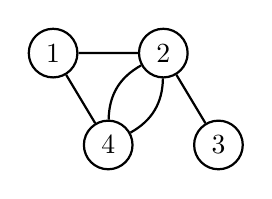
\begin{tikzpicture}[scale=1.4,
  thick,main node/.style={circle,draw,font=\sffamily\bfseries,minimum size=3mm}]

  \node[main node] (1) at (0,15/6) {$1$};
  \node[main node] (2) at (1,15/6){$2$};
  \node[main node] (11) at (1.5,10/6){$3$};
  \node[main node] (12) at (.5,10/6) {$4$};

  \path[every node/.style={font=\sffamily\small}]
  
   (1) edge node{}(2)
   (1) edge node{}(12)
   (2) edge[bend left] node{}(12)
   (2) edge[bend right] node{}(12)
   (2) edge node{}(11)
   (12) edge node{}(12);
\end{tikzpicture}
\end{wrapfigure}

For example, the labeled multigraph $G$ on the diagram has the following Kirchhoff matrix and Kirchhoff minor:
\[A'=\left(
\begin{matrix}
2&-1&0&-1
\\
-1&4&-1&-2
\\
0&-1&1&0
\\
-1&-2&0&3
\end{matrix}
\right),
\quad 
M=\left(
\begin{matrix}
2&-1&0
\\
-1&4&-1
\\
0&-1&1
\end{matrix}
\right).\]

}

\begin{thm}{Exercise}
Show that in any Kirchhoff matrix $A'$ the sum of the components in each row or column vanishes.
Conclude that 
\[\det A'=0.\]

\end{thm}

\begin{thm}{Exercise}
Draw a labeled pseudograph with following Kirchhoff minor:
\[\left(
\begin{matrix}
4&-1&-1&-1&0
\\
-1&4&-1&0&-1
\\
-1&-1&4&-1&-1
\\
-1&0&-1&4&-1
\\
0&-1&-1&-1&4
\end{matrix}
\right).\]
\end{thm}

\begin{thm}{Exercise}\label{ex:sum-kirchhoff}
Show that the sum of all components in every column of Kirchhoff minor is nonnegative.

Moreover, the sum of all components in the $i$-th column vanishes if and only if the $i$-th vertex is not adjacent to the last vertex.
\end{thm}



\parbf{Relabeling.}
Let us understand what happens with Kirchhoff minor and its determinant as we swap two labels distinct from the last one.

\begin{wrapfigure}[6]{o}{28 mm}
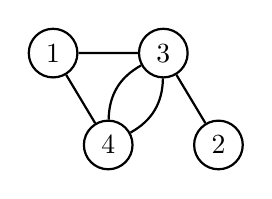
\begin{tikzpicture}[scale=1.4,
  thick,main node/.style={circle,draw,font=\sffamily\bfseries,minimum size=3mm}]

  \node[main node] (1) at (0,15/6) {$1$};
  \node[main node] (2) at (1,15/6){$3$};
  \node[main node] (11) at (1.5,10/6){$2$};
  \node[main node] (12) at (.5,10/6) {$4$};

  \path[every node/.style={font=\sffamily\small}]
  
   
   (1) edge node{}(2)
   (1) edge node{}(12)
   (2) edge[bend left] node{}(12)
   (2) edge[bend right] node{}(12)
   (2) edge node{}(11)
   (12) edge node{}(12);
\end{tikzpicture}
\end{wrapfigure}

For example, if we swap the labels $2$ and $3$ in the graph above,
we get another labeling shown on the diagram.
Then the corresponding Kirchhoff minor will be 
\[
M'=\left(
\begin{matrix}
2&0&-1
\\
0&1&-1
\\
-1&-1&4
\end{matrix}
\right),
\]
which is obtained from $M$ by swapping columns $2$ and $3$ following by swapping rows $2$ and $3$.

Note that swapping a pair of columns or rows changes the sign of the determinant.
Therefore, swapping one pair of rows and one pair of columns does not change the determinant.
Summarizing we get the following:

\begin{thm}{Observation}\label{observaiton:swap}
Assume $G$ is a labeled graph with $p$ vertexes and $M_G$ is its Kirchhoff minor.
If we swap two labels $i,j<p$, then the corresponding Kirchhoff minor $M'_G$ can be obtained from $M_G$ by swapping columns $i$ and $j$, and then swapping rows $i$ and $j$.
In particular, 
\[\det M'_G=\det M_G.\]

\end{thm}

\parbf{Deletion and contraction.}
Let us understand what happens with Kirchhoff minor if we delete or contract an edge in the labeled multigraph.
(If after the contraction of an edge we get loops, we remove it; this way we obtain a multigraph.)

Assume an edge $e$ connects the first and the last vertex of a labeled multigraph $G$ as in the following example:
\begin{center}
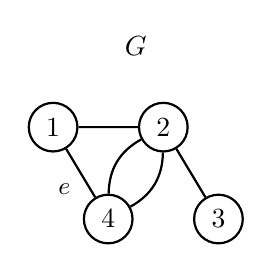
\begin{tikzpicture}[scale=1.4,
  thick,main node/.style={circle,draw,font=\sffamily\bfseries,minimum size=3mm}]

  \node[main node] (1) at (0,15/6) {$1$};
  \node[main node] (2) at (1,15/6){$2$};
  \node[main node] (11) at (1.5,10/6){$3$};
  \node[main node] (12) at (.5,10/6) {$4$};

  \path[every node/.style={font=\sffamily\small}]
  
   (1) edge node{}(2)
   (12) edge node[auto]{$e$}(1)
   (2) edge[bend left] node{}(12)
   (2) edge[bend right] node{}(12)
   (2) edge node{}(11)
   (12) edge node{}(12);
\node[align=center, yshift=2em] (title) 
    at (current bounding box.north)
    {$G$};
\end{tikzpicture}
\hskip5mm
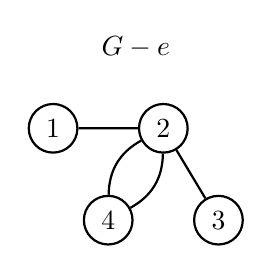
\begin{tikzpicture}[scale=1.4,
  thick,main node/.style={circle,draw,font=\sffamily\bfseries,minimum size=3mm}]

  \node[main node] (1) at (0,15/6) {$1$};
  \node[main node] (2) at (1,15/6){$2$};
  \node[main node] (11) at (1.5,10/6){$3$};
  \node[main node] (12) at (.5,10/6) {$4$};

  \path[every node/.style={font=\sffamily\small}]
  
   (1) edge node{}(2)
   (2) edge[bend left] node{}(12)
   (2) edge[bend right] node{}(12)
   (2) edge node{}(11)
   (12) edge node{}(12);
\node[align=center, yshift=2em] (title) 
    at (current bounding box.north)
    {$G- e$};
\end{tikzpicture}
\hskip10mm
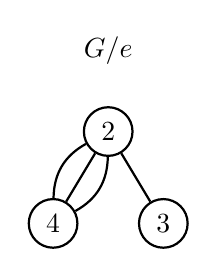
\begin{tikzpicture}[scale=1.4,
  thick,main node/.style={circle,draw,font=\sffamily\bfseries,minimum size=3mm}]

  \node[main node] (2) at (1,15/6){$2$};
  \node[main node] (11) at (1.5,10/6){$3$};
  \node[main node] (12) at (.5,10/6) {$4$};

  \path[every node/.style={font=\sffamily\small}]
  
  (2) edge node{}(12)
   (2) edge[bend left] node{}(12)
   (2) edge[bend right] node{}(12)
   (2) edge node{}(11)
   (12) edge node{}(12);
   \node[align=center, yshift=2em] (title) 
    at (current bounding box.north)
    {$G/e$};
\end{tikzpicture}
\end{center}

Note that deleting $e$ only reduces the corner component of $M_G$ by one,
while contracting it removes the first row and column.
That is, since 
\[M_G=
\left(
\begin{matrix}
2&-1&0
\\
-1&4&-1
\\
0&-1&1
\end{matrix}
\right),\]
we have
\[M_{G- e}=\left(
\begin{matrix}
1&-1&0
\\
-1&4&-1
\\
0&-1&1
\end{matrix}
\right)
\quad\text{and}\quad
M_{G/e}=\left(
\begin{matrix}
4&-1
\\
-1&1
\end{matrix}
\right).\]

Summarizing the above discussion we get the following:

\begin{thm}{Observation}\label{observaiton:dpc}
Assume $e$ is an edge of a labeled multigraph $G$ between the first and last vertex and $M_G$ is the Kirchhoff minor of~$G$.
Then 
\begin{enumerate}[(a)]
\item the Kirchhoff minor  $M_{G- e}$ of $G- e$ can be obtained from  $M_G$ by subtracting 1 from the corner element with index (1,1);
\item the Kirchhoff minor $M_{G/e}$ of $G/e$ can be obtained  from  $M_G$ by removing the first row and the first column in $M_G$.
\end{enumerate}

In particular, applying the cofactor expansion of a determinant, we get that
\[\det M_G=\det M_{G- e}+\det M_{G/ e}.\]

\end{thm}

Note that the last formula resembles the deletion-plus-contraction formula.
This observation will be a key to the proof of the matrix theorem; see the next section.

\section*{Matrix theorem}


\begin{thm}{Matrix theorem}\label{thm:matrix}
Let $M$ be the Kirchhoff minor of a labeled multigraph $G$ with at least two vertexes.
Then
\[s(G)=\det M,\eqlbl{eq:matrix-formula}\]
where $s(G)$ denotes the number of spanning trees in $G$.
\end{thm}


\parit{Proof.}
Denote by $d$ the degree of the last vertex in $G$.

Assume $d=0$.
Then $G$ is not connected and therefore $s(G)=0$.
On the other hand, the sum in each row of $M_G$ vanish (compare to Exercise~\ref{ex:sum-kirchhoff}).
Hence the sum of all columns in $M_G$ vanish;
in particular, the columns in $M_G$ are linearly dependent and hence $\det M_G=0$.
Hence the equality \ref{eq:matrix-formula} holds if $d=0$.

As usual, we denote by $p$ and $q$ the number of vertexes and edges in $G$; by the assumption we have that $p\ge 2$.

\begin{wrapfigure}{o}{25 mm}
\vskip0mm
\centering
\includegraphics{mppics/pic-41}
\end{wrapfigure}

Assume $p=2$; that is, $G$ has two vertexes and $q$ parallel edges connecting them.
Clearly, $s(G)=q$.
Further note that $M_G=(q)$; that is,  the Kirchhoff minor $M_G$ is a $1{\times}1$ matrix with single component $q$.
In particular, $\det M_G=q$ and therefore the equality \ref{eq:matrix-formula} holds.

Assume the equality \ref{eq:matrix-formula} does not hold in general;
choose a graph $G$ that minimize the value $p+q$ among the graphs violating \ref{eq:matrix-formula}.

From above we have that $p>2$ and $d>0$.
Note that we may assume that the first and last vertexes of $G$ are adjacent;
otherwise permute pair of labels $1$ and some $j<p$  and apply Observation~\ref{observaiton:swap}.
Denote by $e$ the edge between the first and last vertex.

Note that the total number of vertexes and edges in the pseudographs $G- e$ and $G/e$ are smaller than $p+q$.
Therefore we have that
\begin{align*}
s(G- e)&=\det M_{G- e},
&
s(G/e)&=\det M_{G/e}.
\end{align*}
Applying these two identities together with the deletion-plus-contraction formula 
and Observation~\ref{observaiton:dpc}, we get that
\begin{align*}
s(G)&=s(G- e)+s(G/e)=
\\
&=\det M_{G- e}+\det M_{G/e}=
\\
&=\det M_G;
\end{align*}
that is, the identity \ref{eq:matrix-formula} holds for $G$ --- a contradiction.
\qeds


\begin{thm}{Exercise}
Fix a labeling for each of the following graphs, 
find its Kirchhoff minor and use the matrix theorem to find the number of spanning trees.
\begin{enumerate}[(a)]
\item $s(K_{3,3})$;
\item $s(W_6)$;
\item $s(Q_3)$.
\end{enumerate}
(Use \href{https://matrix.reshish.com/determinant.php}{\emph{\texttt{https://matrix.reshish.com/determinant.php}}}, or any other matrix calculator.)
\end{thm}


\section*{Calculation of determinants}

In this section we recall key properties of the determinant which will be used in the next section.

Let $M$ be an $n{\times}n$-matrix; that is, a table $n{\times}n$, filled with numbers which are called {}\emph{components of the matrix}.
The determinant $\det M$ is a polynomial of the $n^2$ components of $M$,
which satisfies the following conditions:
\begin{enumerate}
 \item\label{1} The unit matrix has determinant 1; that is,
\[
\det\left(
\begin{matrix}
1&0&\cdots&0
\\
0&1&\ddots&\vdots
\\
\vdots&\ddots&\ddots&0
\\
0&\cdots&0&1
\end{matrix}
\right)=1.
\]
\item\label{2} If we multiply each component of one of the rows of the matrix $M$ multiply by a number $\lambda$, then for the obtained matrix $M'$, we have
\[\det M'=\lambda\cdot \det M.\]

\item\label{3} If one of the rows in the matrix $M$ add (or subtract) term-by-term to another row, then the obtained matrix $M'$ has the same determinant
\[\det M'= \det M.\]
\end{enumerate}
These three conditions define determinant in a unique way. 
We will not give a proof of the statement; it is not evident and not complicated (sooner or later you will have to learn it, if it is not done already).

\begin{thm}{Exercise}
Show that the following property follows from the properties above.
\end{thm}

\begin{enumerate}[resume]
 \item Interchanging any pair of rows of a matrix multiplies its determinant by $-1$; that is, if a matrix $M'$ is obtained from a matrix $M$ by permuting two of its rows, then 
\[\det M'=-\det M.\]
\end{enumerate}

The determinant of $n\times n$-matrix can be written explicitly as a sum of $n!$ terms. 
For example, 
\[
a_1{\cdot} b_2{\cdot} c_3+a_2{\cdot} b_3{\cdot} c_1+a_3{\cdot} b_1{\cdot} c_2-a_3{\cdot} b_2{\cdot} c_1-a_2{\cdot} b_1{\cdot} c_3-a_1{\cdot} b_3{\cdot} c_2\]
is the determinant of the matrix
\[M=\left(
\begin{matrix}
a_1&b_1&c_1
\\
a_2&b_2&c_2
\\
a_3&b_3&c_3
\end{matrix}
\right).\]
However, the properties described above give a more convenient and faster way to calculate the determinant, especially for larger values~$n$.

Let us show it on one example which will be needed in the next section.
\begin{align*}
\det\left(
\begin{matrix}
4&-1&-1&-1
\\
-1&4&-1&-1
\\
-1&-1&4&-1
\\
-1&-1&-1&4
\end{matrix}
\right)
=
&\det\left(
\begin{matrix}
1&1&1&1
\\
-1&4&-1&-1
\\
-1&-1&4&-1
\\
-1&-1&-1&4
\end{matrix}
\right) 
=
\\
=
&\det\left(
\begin{matrix}
1&1&1&1
\\
0&5&0&0
\\
0&0&5&0
\\
0&0&0&5
\end{matrix}
\right)
=
\\
=
5^3\cdot
&\det\left(
\begin{matrix}
1&1&1&1
\\
0&1&0&0
\\
0&0&1&0
\\
0&0&0&1
\end{matrix}
\right)=
\\
=
5^3\cdot&\det\left(
\begin{matrix}
1&0&0&0
\\
0&1&0&0
\\
0&0&1&0
\\
0&0&0&1
\end{matrix}
\right)=
\\
=5^3&.
\end{align*}
Let us describe what we used on each line above:
\begin{enumerate}
\item property \ref{3} three times --- we add to the first row each of the remaining rows;
\item property \ref{3} three times --- we add the first row to the each of the remaining three rows;
\item property \ref{2} three times;
\item property \ref{3} three times --- we subtract from the first row the remaining three rows;
\item property \ref{1}.
\end{enumerate}


\section*{Cayley formula}

Recall that a \index{complete graph}\emph{complete graph} is a graph where each pair of vertexes is connected by an edge;
a complete graph with $p$ vertexes is denoted by~$K_p$.

Note that every vertex of $K_p$ has degree $p-1$.
Therefore the Kirchhoff minor $M=M_{K_p}$ in the matrix formula \ref{eq:matrix-formula} for $K_p$ is the following $(p-1)\times (p-1)$-matrix:

\[
M=\left(
\begin{matrix}
p{-}1&-1&\cdots&-1
\\
-1&p{-}1&\ddots&\vdots
\\
\vdots&\ddots&\ddots&-1
\\
-1&\cdots&-1&p{-}1
\end{matrix}
\right).
\]

The argument given in the end of the previous section admits a direct generalization:
\begin{align*}
\det\left(
\begin{matrix}
p{-}1&-1&\cdots&-1
\\
-1&p{-}1&\ddots&\vdots
\\
\vdots&\ddots&\ddots&-1
\\
-1&\cdots&-1&p{-}1
\end{matrix}
\right)
&=\det\left(
\begin{matrix}
1&1&\cdots&1
\\
-1&p{-}1&\ddots&\vdots
\\
\vdots&\ddots&\ddots&-1
\\
-1&\cdots&-1&p{-}1
\end{matrix}
\right)
=
\\
&=
\det\left(
\begin{matrix}
1&1&\cdots&1
\\
0&p&\ddots&\vdots
\\
\vdots&\ddots&\ddots&0
\\
0&\cdots&0&p
\end{matrix}
\right)=
\\
&=  p^{p-2}.
\end{align*}
That is,
\[\det M=p^{\,p-2}.\]
Therefore, applying the matrix theorem, we get the following:

\begin{thm}{Cayley formula}\label{thm:cayley}
 \[s(K_p)=p^{p-2};\]
that is, the number of spanning trees in the complete graph $K_p$ is $p^{p-2}$.
\end{thm}

\begin{thm}{Exercise}
Use the matrix theorem to show that 
\[s(K_{m,n})=m^{n-1}\cdot n^{m-1}.\]
\end{thm}



\section*{Remarks}

There is strong connection between counting spanning trees of a given graph,
calculations of currents in an electric chain 
and random walks; a good survey is given in the book of Peter Doyle and Laurie Snell \cite{doyle-snell}. Let us give some examples.

Assume that the graph $G$ describes an electric chain;
each edge has resistance one Ohm and a battery is connected to the vertexes $a$ and $b$.
Assume that the total current between these vertexes is one Ampere and we need to calculate the current thru a given edge $e$.

Fix an orientation of $e$.
Note that any spanning tree $T$ of $G$ has exactly one the following three properties:
(1) the edge $e$ appears on the (necessary unique) path from $a$ to $b$ in $T$ with a positive orientation,
(2) the edge $e$ appears on the path from $a$ to $b$ in $T$ with a negative orientation,
(3) the edge $e$ does not appear on the path from $a$ to $b$ in $T$.
Denote by $s_+$, $s_-$, and $s_0$ the number of the trees in each group.
Clearly,
\[s(G)=s_++s_-+s_0.\]

The current $I_e$ along $e$ can be calculated using the following formula:
\[I_e=\frac{s_+-s_-}{s(G)}\cdot I.\]
This statement can be proved by checking Kirchhoff's rules for the currents calculated by this formula.

There are many other applications of Kirchhoff's rules to graph theory.
For example, in \cite{levi}, they were used to prove the Euler's formula
\[p-q+r=2,\]
where $p$, $q$, and $r$ denote the number of vertexes, edges and regions of in a plane drawing of graph.

A few interesting proofs of Cayley formula are given in \cite[Chapter 30]{aigner-ziegler};
the most popular proof using the Pr\"ufer's code is given in \cite{hartsfield-ringel}.



